\documentclass[journal]{IEEEtran}
\usepackage[
backend=biber,
style=alphabetic,
sorting=ynt
]{biblatex}
\addbibresource{mybibliography.bib}

\title{Bibliography management: \texttt{biblatex} package}
\author{Share\LaTeX}
\date{ }
\usepackage{amsmath,epsfig,,amssymb}
\usepackage{graphicx}
\usepackage{tikz}
%\usepackage{pgfplots}
\usepackage{mathtools}
\usepackage{multirow}
%\usepackage{subcaption}
\usepackage[caption=false, font=footnotesize]{subfig}
\usepackage{mathtools}
\usepackage{cuted}
\usepackage[linesnumbered,ruled,vlined]{algorithm2e}
\def\x{{\mathbf x}}
\def\L{{\cal L}}
\ifCLASSINFOpdf
\else
\fi

\hyphenation{op-tical net-works semi-conduc-tor}

\begin{document}

\title{BetterProctor: Next Gen Proctoring Solution}
\author{Tarun Mali,\IEEEmembership{ Perin Mangukiya,}\IEEEmembership{ Ajay Kumbhar},\IEEEmembership{ Hari Jarupla}}% <-this % stops a space
\vspace{-0.5cm}
%\thanks{(Corresponding author: Manjunath V.~Joshi)}
%\thanks{J. R. Patel (e-mail: jignnesh@gmail.com) and M. V. Joshi (e-mail:mv\_joshi@daiict.ac.in) are with Dhirubhai Ambani Institute of Information and Communication Technology (DA-IICT), Gandhinagar 382007, India.}% <-this % stops a space
%\thanks{J. S. Bhatt (e-mail: jignesh.bhatt@iiitvadodara.ac.in) is with Indian Institute of Information Technology Vadodara (IIITV),Gandhinagar 382027, India.}
%}

%\markboth{IEEE JOURNAL OF SELECTED TOPICS IN APPLIED EARTH OBSERVATIONS AND REMOTE SENSING.}
%%\markboth{Journal of \LaTeX\ Class Files,~Vol.~14, No.~8, August~2015}%
%{Shell \MakeLowercase{\textit{et al.}}: Bare Demo of IEEEtran.cls for IEEE Journals}
\maketitle

\begin{abstract} 
Current Proctoring solutions are often prone to errors and can be
costly to maintain. This project aims to develop a proctoring website
that using TensorFlow.js to detect the person taking the exam in real-time. 

One of the key advantages of this proctoring website is that it
runs entirely in the browser by using TensorFlow.js . This eliminates
the need for sending the video feed back to the server or running
computationally expensive ML models in the back-end thus reducing
a ton on computing resources and hence lowering the server costs.
Additionally, running the machine learning models in the browser will
give more control on the data, as all the data will be processed on
the user’s device, giving more security and privacy.The Proctoring
solution will also have a provision in which the invigilator can video
call the candidate in real time if the “Trust-Score” of the candidate
falls below a certain threshold. The Video-Call will be based on a P2P
architecture and also does not require any additional back-end as the
video streams will flow directly between the browsers.\\

\end{abstract}

\begin{IEEEkeywords}
 Browser Proctoring, TensorFlow.js, Facial recognition, Deep learning, P2P.
\end{IEEEkeywords}

\IEEEpeerreviewmaketitle

\section{Introduction }
Proctoring software is an essential tool for ensuring the integrity of online exams.However, current solutions are often prone to errors and can be costly to maintain. This project aims to develop a proctoring website that using TensorFlow.js to detect the person taking the exam in real-time. The website will use facial recognition to ensure the identity of the person taking the exam, providing a secure and efficient solution for online proctoring.\\


One of the key advantages of this proctoring website is that it runs entirely in the browser by using TensorFlow.js. TensorFlow.js is a JavaScript library that allows you to create and run machine learning models in the browser without any installation or setup. This eliminates the need for sending the video feed back to the server or running computationally expensive ML models in the backend thus reducing a ton on computing resources and hence lowering the server costs. By running the ML models in the browser, you can also leverage the power of the user's device and optimize the performance and accuracy of the proctoring system. Additionally, running the machine learning models in the browser will give more control on the data, as all the data will be processed on the user’s device, giving more security and privacy. This way, you can ensure that no sensitive information is leaked or compromised during the proctoring process. Furthermore, running the ML models in the browser will also enable offline proctoring, which means that you can conduct exams even when there is no internet connection available. This will increase the accessibility and convenience of online proctoring for both students and instructors.\\


One of the main goals of this proctoring website is to ensure the integrity and validity of online exams by detecting and preventing any cheating attempts. To achieve this, the website will utilize deep learning techniques, as TensorFlow.js is a powerful tool for building and deploying machine learning models, including deep learning models, in the browser. Facial recognition, which is a key feature of the website, is a task that can be accomplished using deep learning algorithms such as convolutional neural networks. These algorithms can learn to recognize and verify the identity of the test takers by analyzing their facial features and expressions. This will make the system more accurate and reliable as it will be harder to bypass as the data is not transmitted over the internet. \\


Instead, the processing is done locally on the user's device, ensuring privacy and security. The website will also use other deep learning techniques to monitor the test takers' behavior and environment, such as eye tracking, head pose estimation, and background noise detection. These techniques will help to identify any suspicious or abnormal activities that may indicate cheating or distraction. By using TensorFlow.js and deep learning techniques, this proctoring website will provide a robust and convenient solution for online exam proctoring.\\


One of the challenges of machine learning (ML) is to make it accessible and easy to use for a wide range of developers. While most of the production-quality ML libraries are designed for Python and C++ developers, there is a huge demand for ML solutions in the web domain, where JavaScript (JS) is the dominant programming language. JS has a large and active developer community, as evidenced by the number of GitHub pull requests and Stack Overflow questions related to JS in recent years. To bridge the gap between ML and web development, TensorFlow.js was created as a library that allows JS developers to create, train, and deploy ML models in the browser or on Node.js servers. TensorFlow.js leverages the power of WebGL and WebAssembly to run computations on the GPU or CPU, respectively. TensorFlow.js also provides a variety of tools and APIs to help developers with different levels of ML expertise to build and deploy ML applications on the web.\\

TensorFlow.js is a powerful and versatile framework for machine learning and numerical computation in JavaScript. It allows developers to create and deploy ML models in the browser, on the server, or on the edge using WebGL and Node.js. TensorFlow.js is compatible with the TensorFlow ecosystem, enabling seamless interoperability with other TensorFlow tools and libraries. TensorFlow.js also provides a rich set of APIs and tools for building, training, and deploying ML models in JS environments. TensorFlow.js is not just another JS library for ML, but a comprehensive platform that leverages the GPU and the JS community to deliver high performance and user-friendly ML solutions.\\

Our solution is designed to ensure the integrity and validity of online examinations. We use real-time proctoring to monitor the candidates' behavior and environment during the test. We also assign a "Trust-Score" to each candidate based on various parameters such as eye movement, face detection, audio analysis, and screen activity. If the "Trust-Score" falls below a certain threshold, indicating a possible cheating attempt, the invigilator can initiate a video call with the candidate in real time. The video call will allow the invigilator to verify the identity of the candidate and ask them to show their surroundings. The video call will be based on a peer-to-peer (P2P) architecture, which means that the video streams will flow directly between the browser of the invigilator and the candidate. This will ensure a high-quality and low-latency communication without requiring any additional backend infrastructure or bandwidth. \\

In conclusion, this proctoring website represents a significant advancement in the field of online proctoring. By running entirely in the browser and utilizing deep learning techniques, it offers a more efficient, secure, and cost-effective solution than current proctoring software. This makes it a valuable tool for educational institutions, businesses, and other organizations that need to ensure the integrity of online exams. The website has several features that distinguish it from its competitors, such as facial recognition, eye tracking, keystroke analysis, and browser lockdown. These features enable the website to detect and prevent any cheating attempts during the exam, while also ensuring the privacy and comfort of the test-takers. The website also provides detailed reports and analytics for the exam administrators, allowing them to monitor and evaluate the performance and behavior of the test-takers. The website is easy to use and compatible with various devices and browsers, making it accessible and convenient for both exam administrators and test-takers. The website is also scalable and reliable, capable of handling large numbers of concurrent exams without compromising on quality or security. The website is therefore a promising innovation that can revolutionize the field of online proctoring and enhance the credibility and validity of online exams.



\section{Related work}
Given the popularity and the unique benefits of the JS ecosystem, it is no surprise that many open-source browser-based ML libraries exist. ConvNetJS (Karpathy, 2014)~\cite{1}, Synaptic (Cazala, 2014)~\cite{2}, Brain.js (Plummer, 2010)~\cite{3}, Mind (Miller, 2015)~\cite{4} and Neataptic (Wagenaar, 2017)~\cite{5} each provide a simple JS API that allows beginners to build and train neural networks with only a few lines of code. More specialized JS ML libraries include Compromise (Kelly, 2014)~\cite{6} and Natural (Umbel, 2011)~\cite{7}, which focus on NLP applications, and NeuroJS (Huenermann, 2016)~\cite{8} and REINFORCEjs (Karpathy, 2015)~\cite{9}, which focus on reinforcement learning. ML.js (Zasso, 2014)~\cite{10} provides a more general set of ML utilities, similar to the Python-based scikit-learn (Pedregosa et al., 2011)~\cite{11}.\\\\
There are several proctoring software solutions available today that are used for online
exams and assessments.\\\\
1. ProctorU: This is a cloud-based proctoring solution that uses live human proctors to
monitor exams in real-time.\\
2. Respondus: This is a software that integrates with learning management systems to
provide a secure and automated proctoring experience.\\
3. ExamSoft: This is a comprehensive exam management software that includes
proctoring features such as real-time monitoring and flagging of suspicious
behavior.\\
4. Honorlock: This is a cloud-based proctoring solution that uses artificial intelligence
to monitor exams and detect suspicious behavior.\\
5. SofTest: This is a software that allows students to take exams on their own
computer while Most of the existing proctoring software solutions perform the AI
processing on the server side.\\\\
Most of the existing proctoring software solutions perform the AI processing on the
server side. This means that the software uses specialized hardware and infrastructure to process the data and perform the AI analysis. For example, ProctorU uses live
human proctors to monitor exams in real-time, while Respondus integrates with learning
management systems to provide a secure and automated proctoring experience.
Honorlock uses artificial intelligence to monitor exams and detect suspicious behavior,
but this processing is done on the server side.\\
\section{Problem statement }
One of the main challenges of online education is ensuring academic integrity. To prevent cheating and plagiarism, many online courses use proctoring solutions that monitor students' behavior during exams. However, the current proctoring solutions available in the market rely heavily on face recognition technology. These solutions employ machine learning models that run in the cloud or backend. However, the process of running these models is computationally expensive, making the proctoring solution expensive for colleges to purchase. Moreover, these solutions raise privacy and ethical concerns, as they collect and store sensitive data from students' faces and environments.\\

 
Face recognition technology has the potential to enhance the security and quality of online exams by verifying the identity of test-takers and detecting any cheating attempts. However, many educational institutions face a significant challenge in adopting such technology due to the high cost of existing proctoring solutions. These solutions often require expensive hardware, software, and human resources to monitor and review the exam sessions. This may limit the access and affordability of online education for many students and educators. Therefore, there is a need for more cost-effective and scalable face recognition solutions that can provide reliable and accurate proctoring services for online exams.\\

One possible way to address this problem is to use a hybrid approach that combines face recognition with other biometric modalities, such as voice or fingerprint recognition. This way, the system can verify the identity of the test taker using multiple sources of evidence, reducing the reliance on face recognition alone. Moreover, by using efficient algorithms and cloud-based services, the system can reduce the computational costs and bandwidth requirements of proctoring exams online. Such a system would provide a cost-effective and secure solution for educational institutions that want to ensure exam integrity without compromising on quality or accessibility.

\section{Problem formulation }
\subsection{Detail 1:} 
One possible solution to this problem is to develop a biometric authentication system that verifies the identity of the students taking the exams. The system would use facial recognition, voice recognition, and keystroke dynamics to ensure that the students are who they claim to be and that they are not using any unauthorized resources. The system would also monitor the students' behavior during the exams and flag any suspicious activities, such as looking away from the screen, talking to someone else, or switching tabs. The system would be computationally efficient, scalable, and reliable, as it would use cloud-based services and machine learning algorithms to process and analyze the biometric data. The system would also be user-friendly and easy to integrate with existing educational technology platforms, as it would require minimal hardware and software installation and configuration. The system would only need a webcam, a microphone, and a browser extension to work. The system would be affordable for educational institutions, as it would use a pay-per-use model and offer discounts for bulk purchases. The system would prevent cheating during exams and ensure academic integrity and fairness.

\subsection{Detail 2:}
Online proctoring systems (OPS) are technology-enabled services that allow remote monitoring of online exams and assessments. One of the key features of OPS is face recognition technology, which can verify the test taker's identity and detect any suspicious behavior during the exam. However, face recognition technology requires high computational costs, which makes OPS expensive for colleges to purchase. Therefore, the problem is to develop a cost-effective proctoring solution that can employ face recognition technology without the high computational costs


\section{Proposed Approach : }
Proctoring is a process of monitoring and verifying the identity and behavior of test-takers in online exams. Proctoring solutions often rely on cloud or backend computing to run machine learning models that analyze the video and audio streams of the test-takers. However, this approach has some drawbacks, such as high costs, data privacy risks, and dependency on internet speed and availability.

One possible solution to the problem of expensive proctoring solutions is to use TensorFlow.js in the browser to run the machine learning model instead of relying on cloud or backend computing. This approach offers several advantages, including data privacy, accessibility, low-latency, and cost savings.

By running the machine learning model in the browser, data privacy concerns can be addressed since sensitive data does not have to leave the user’s device. This approach also makes the solution more accessible to users since it does not require a high-speed internet connection or access to a cloud or backend service. Moreover, running the model in the browser reduces the latency and improves the performance of the proctoring solution. Finally, this approach can save costs for both test-takers and test-providers since they do not have to pay for cloud or backend computing resources.\\

One of the benefits of using TensorFlow.js in the browser is that it can provide a proctoring solution that respects data privacy and accessibility. By running the machine learning model in the browser, the exam data does not need to be sent to a third-party server, which reduces the risk of data breaches or misuse. Furthermore, this approach can also accommodate different devices and browsers, making the proctoring solution more accessible to a diverse range of students. Another advantage of using TensorFlow.js in the browser is that it can improve the performance and affordability of the proctoring solution. By leveraging the computational power of the browser, the machine learning model can run faster and more smoothly, resulting in a lower latency and a better user experience. Additionally, this approach can also reduce the costs associated with cloud or backend computing, which makes the proctoring solution more economical for educational institutions. In summary, using TensorFlow.js in the browser can offer a proctoring solution that is cost-effective and efficient, while also ensuring exam integrity and addressing data privacy and accessibility issues.


To extract features using MobileNet, we can use the pre-trained model provided by TensorFlow.js, which has been trained on a large-scale image classification task such as ImageNet. The MobileNet model can be loaded using the tf.loadGraphModel() function, and then used to extract features from input images or video frames using the model.predict() function. The predict() function returns a 2D tensor of shape (N, 1024), where N is the number of input images or video frames, and 1024 is the number of output features from the final convolutional layer of MobileNet.\\

By using the k-NN algorithm to classify the features extracted by the MobileNet architecture, it is possible to create an efficient and accurate autoproctoring system that can recognize and classify body postures in real-time video.\\

The k-NN algorithm is a type of instance-based learning that works by finding the k-nearest neighbors to a given input data point in the feature space, and then assigning the class label of the majority of those neighbors to the input point.

\section{Implementation : }
Implementation steps for a machine learning model that uses TensorFlow.js library to recognize and classify body postures in real-time video using MobileNet architecture and KNN classifier:

Collect and preprocess data: To train the model, you will need to collect a dataset of labeled images or video frames of different body postures. You can use a webcam or a pre-recorded video to capture the data. Then, you will need to preprocess the data by resizing and normalizing the images or video frames.

Load MobileNet model: TensorFlow.js provides a pre-trained MobileNet model that can be used as a feature extractor for body posture recognition. You can load the MobileNet model using the tf.loadGraphModel() function. 

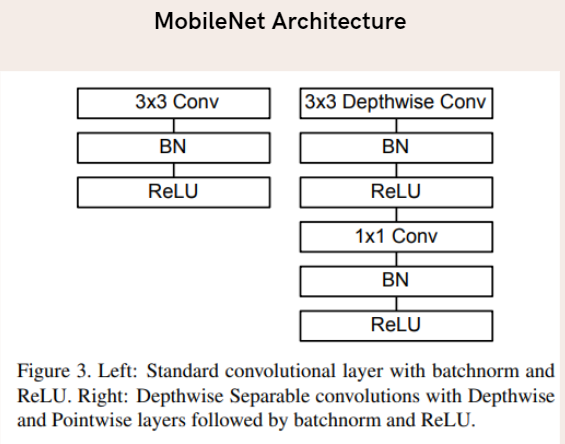
\includegraphics[width=0.4\textwidth]{img1.png}





Extract features: Once you have loaded the MobileNet model, you can use it to extract features from the preprocessed images or video frames. The MobileNet model outputs a 1024-dimensional feature vector for each image or video frame, which represents the high-level features of the image.

Train KNN classifier: After extracting the features, you will need to train a K-Nearest Neighbors (KNN) classifier to recognize and classify different body postures. KNN is a simple yet effective classification algorithm that works well with high-dimensional feature vectors. You can use the tf.KNNeighborsClassifier() function to create a KNN classifier and train it using the extracted features and their corresponding labels.

Test the model: Once the model is trained, you can test it on real-time video streams using TensorFlow.js and a webcam. You can use the navigator.mediaDevices.getUserMedia() function to access the webcam and capture real-time video frames. Then, you can preprocess the frames, extract features using the MobileNet model, and classify the body posture using the trained KNN classifier.

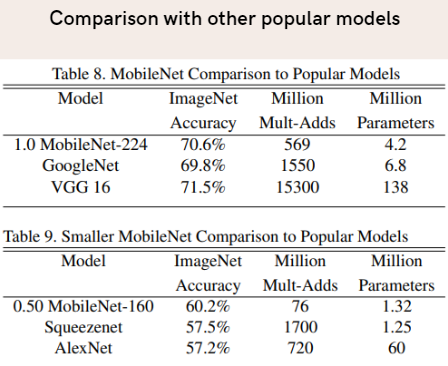
\includegraphics[width=0.4\textwidth]{img2.png}


Deploy the model: Finally, you can deploy the model as a web application using TensorFlow.js and a web server. You can use the tfjs-converter tool to convert the TensorFlow.js model to a format that can be used in a web application, and then load the model using the tf.loadGraphModel() function in the client-side JavaScript code.

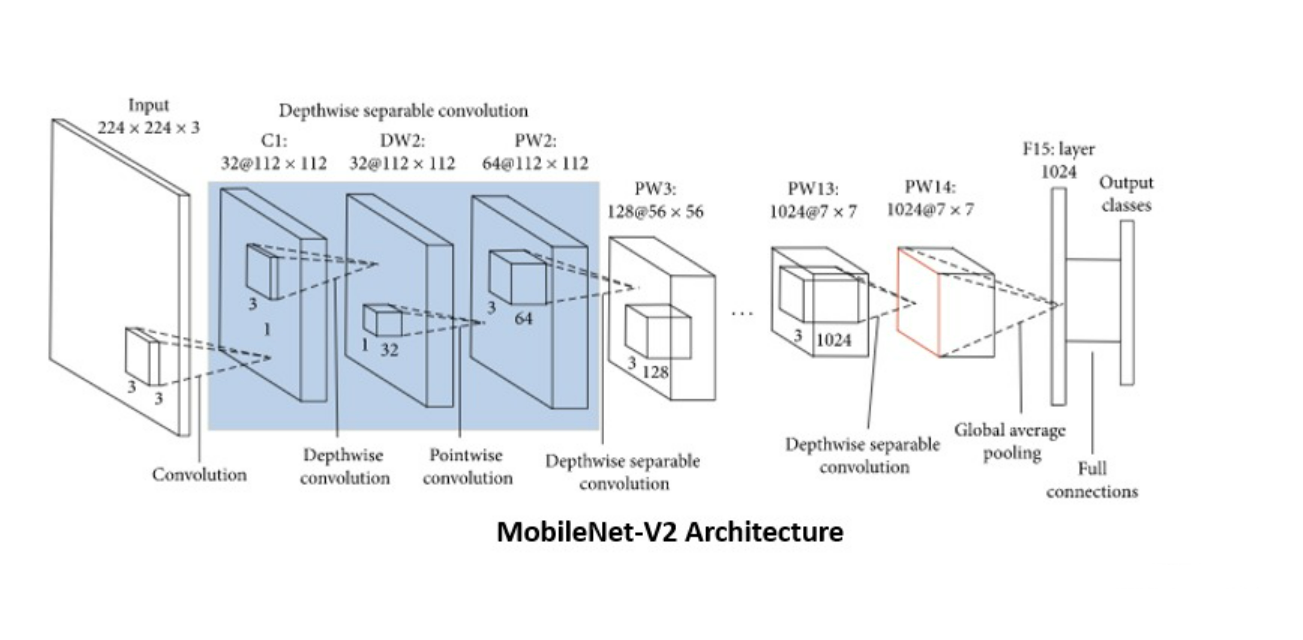
\includegraphics[width=0.5\textwidth]{mobileNet_final.png}


\subsection{Additional features :}
1. \textbf{Audio Detection} : For recording a student's speech for a certain amount of time (10 seconds in this case), converting the recorded audio to text using Google's speech recognition API, and comparing the text with a set of predefined questions (stored in a separate file) to determine whether the student needs to be alerted to a potential violation.

Implementation : 
The code uses the PyAudio library to record audio and the SpeechRecognition library to convert speech to text using Google's speech recognition API. It saves the converted text to a file called "test.txt". It then reads the file and removes stop words using the NLTK library. The resulting filtered text is saved to a new file called "final.txt".

The code also reads a file called "paper.txt" containing the predefined questions, removes stop words from the questions, and compares them with the filtered text obtained from the student's speech. If there are any common words between the questions and the student's speech, it prints the number of common elements and the common elements themselves. The code does not contain any specific logic for determining whether a violation has occurred or not.

Speech Recognition Model:
The $speech_recognition$ library is used to perform speech recognition on audio files. It uses deep learning models to transcribe the speech from the audio input into text. Specifically, the $recognize_google$ function uses Google's Cloud Speech API, which employs deep neural networks to perform speech recognition.

Text Processing Models:
The code uses the $nltk$ library for natural language processing tasks such as $tokenization$, stop-word removal, and filtering. The library uses various machine learning models and algorithms for these tasks, such as the $stopwords$ corpus and $word_tokenize$ function. These models are based on deep learning algorithms such as neural networks and decision trees.

Overall, the code makes use of various deep learning models to perform speech-to-text conversion and text processing tasks.



2. \textbf{Face Detection} : BlazeFace is an object detection algorithm designed to detect faces in real-time, developed by Google researchers.BlazeFace is built on top of the Single Shot Multibox Detector (SSD) architecture and uses depthwise separable convolutions to reduce the number of parameters and computational complexity. The model is trained on the WIDER FACE dataset, which contains over 32,000 images with over 50,000 labeled faces.


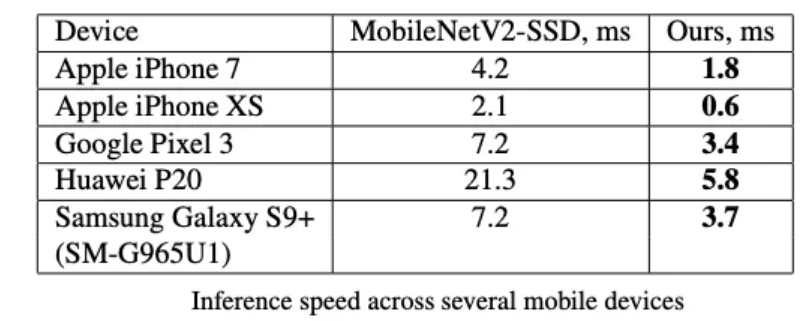
\includegraphics[width=0.4\textwidth]{blaze.png}

The deep learning theory behind BlazeFace involves the use of convolutional neural networks (CNNs) for object detection. CNNs consist of multiple layers of convolutional and pooling operations, followed by fully connected layers for classification. The convolutional layers learn to extract features from the input images, while the pooling layers downsample the feature maps to reduce the spatial dimensionality. The fully connected layers perform the final classification.

BlazeFace uses a feature pyramid network (FPN) to handle faces of different sizes and scales. The FPN consists of a base network that generates a feature map, followed by multiple layers that refine the feature map at different scales. The output of the FPN is a set of feature maps that are fed into the object detection module.

The object detection module in BlazeFace uses anchor boxes to predict the location and size of faces in the input image. The anchor boxes are pre-defined boxes of different sizes and aspect ratios that are used to generate candidate regions for face detection. The CNN predicts the offset and scale of each anchor box to generate the final bounding box predictions.

Overall, the deep learning theory behind BlazeFace involves the use of CNNs and FPNs for feature extraction and object detection, along with anchor boxes for bounding box prediction. The model is trained on a large dataset of labeled faces and optimized for real-time performance on low-power devices.







\bibliographystyle{IEEEtran}
\begin{thebibliography}{10}
\bibitem{1}
  Karpathy, A. ConvNetJS: Deep learning in your browser. http://cs.stanford.edu/people/
karpathy/convnetjs, 2014. Accessed: 2018-08-
25.\\
\bibitem{2}
Cazala, J. Synaptic. https://github.com/cazala/
synaptic, 2014. Accessed: 2018-08-25.\\
\bibitem{3}
Plummer, R. brain.js. https://github.com/
BrainJS/brain.js, 2010. Accessed: 2018-08-25.\\
\bibitem{4}
Miller, S. Mind. https://github.com/
stevenmiller888/mind, 2015. Accessed:
2018-08-25.\\
\bibitem{5}
Wagenaar, T. Neataptic. https://github.com/
wagenaartje/neataptic, 2017. Accessed: 2018-
08-25.\\
\bibitem{6}
Kelly, S. compromise. https://github.com/
spencermountain/compromise, 2014. Accessed:
2018-08-25..\\
\bibitem{7}
Umbel, C. Natural. https://github.com/
NaturalNode/natural, 2011. Accessed: 2018-08-
25.\\
\bibitem{8}
Huenermann, J. neurojs. https://github.com/
janhuenermann/neurojs, 2016. Accessed: 2018-
08-25.\\
\bibitem{9}
Karpathy, A. REINFORCEjs: Reinforcement learning
agents in javascript. https://github.com/
karpathy/reinforcejs, 2015. Accessed: 2018-
08-25.\\
\bibitem{10}
Zasso, M. ml.js. https://github.com/mljs/ml,
2014. Accessed: 2018-08-25.\\
\bibitem{11}
Pedregosa, F., Varoquaux, G., Gramfort, A., Michel, V.,
Thirion, B., Grisel, O., Blondel, M., Prettenhofer, P.,
Weiss, R., Dubourg, V., Vanderplas, J., Passos, A., Cournapeau,
D., Brucher, M., Perrot, M., and Duchesnay, E.
Scikit-learn: Machine learning in Python. Journal of
Machine Learning Research, 12:2825–2830, 2011 \\
\bibitem{12}
Speech-to-Text: Automatic Speech Recognition  |  Google Cloud (2023). Available at: https://cloud.google.com/speech-to-text (Accessed: 14 April 2023).\\
\bibitem{13}
Bazarevsky, V., Kartynnik, Y., Vakunov, A., Raveendran, K. and Grundmann, M.
Bazarevsky, V. et al. (2019) BlazeFace: Sub-millisecond Neural Face Detection on Mobile GPUs, arXiv.org. Available at: https://arxiv.org/abs/1907.05047 (Accessed: 14 April 2023).\\
\bibitem{13}
NLTK :: Natural Language Toolkit
NLTK :: Natural Language Toolkit (2023). Available at: https://www.nltk.org/ (Accessed: 14 April 2023).\\





\end{thebibliography}

\vspace{-1cm}
\end{document}